%!TEX root = main.tex
\section{Performance}
    At this point we started some simulations to check various performances. We mentioned in section \ref{sec:model_eval} that the models Logistic Regression, Random Forest and MLP were left over. Before we started the simulations we performed a few tests. The three models calculated probabilities for a specific market situation. Also a set of training data was given. MLP calculated probabilities which seemed not to be realistic. However, Logistic Regression and Random Forest showed good results. Therefore, we decided to not focus on MLP any more and compare the performance of Logistic Regression and Random Forest in the simulations.

\subsection{Pricewars Platform}
    In the winter term 2016/17 a master's project from the HPI has built a simulation platform. The main goal of this platform is to evaluate how different pricing strategies perform. Essentially, the platform is a marketplace environment where customers exist. The customers have behaviours that can be configured. Several merchants are already implemented as well. Thus, it is easy to let our own merchant compete against others. The application is based on a microservice architecture. Each merchant has an authentication token and REST requests are used to communicate.

\subsection{Simulations}
    We start the existing merchants Two Bound, Cheapest and Fix Price for the following simulations. The consumer performs 100 purchases per minute and is set to 100\% logit behaviour. The logit coefficients are shown in figure \ref{fig1}.
    \begin{figure}[ht]
    \centering
        \begin{tabular}{ l | c | r | r | r}
            interc. & price rank & amount competitors & avg price & quality rank \\
            \hline  
            -6.62 & 0.2 & 0.25 & -0.008 & -0.18 \\
        \end{tabular}
    \caption{Logit coefficients}
    \label{fig1}
    \end{figure}

    The universal model (section \ref{sec:universal_model}) is not used during the simulations. Because of that the charts can illustrate the learning effect of our approach better. Instead of the universal model the merchant sets random prices for the first learning interval. Thereby it generates an accurate training data set for the following price predictions. One learning interval takes two minutes. Figure \ref{fig2} shows that Random Forest chooses prices between 0.8 times and 3 times the purchase price (see section \ref{sec:random_prices}). The prices from the Cheapest and the Two Bound merchants are also influenced by the random prices. This interval is called exploration phase.
    
    \begin{figure}[ht]
        \centering
        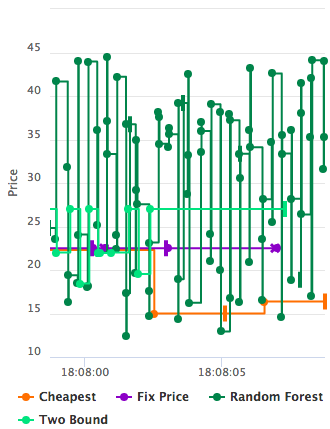
\includegraphics[width=0.35\textwidth]{img/rndmfrst_explor2.png}
        \caption{Price chart exploration phase}
        \label{fig2}
    \end{figure}
 

\subsubsection{Logistic Regression Simulation}
    ~\\
    The Logistic Regression simulation begins with the exploration phase. This phase is similar to the Random Forest exploration phase from figure \ref{fig2}. Afterwards, the model has collected enough training data and the new best prices are predicted by the Logistic Regression model. You can see in figure \ref{fig3} that our merchants predicts the highest possible price as best price.

    \begin{figure}[ht]
        \centering
      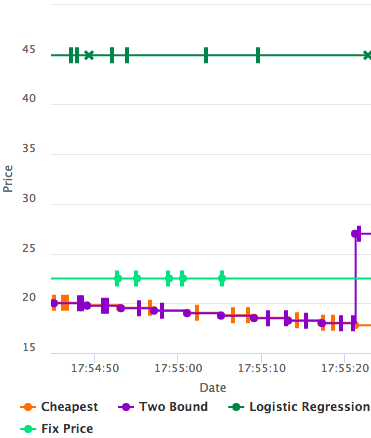
\includegraphics[width=0.35\textwidth]{img/logit_prices.png}
        \caption{Price chart Logistic Regression}
        \label{fig3}
    \end{figure}
 


\subsubsection{Random Forest Simulation}

    
\subsection{Drawbacks}
